\section{Obtención de los parámetros $q_{1}$ y $q_{2}$}

En esta sección vamos a explicar cómo obtuvimos los valores de $q_{1}$ y $q_{2}$. Son parámetros que se introducen en la función \textit{hw()} de \textit{R}. Representan los cuantiles utilizados al calcular los intervalos de confianza. Por ejemplo si $q_{1} = 80$ entonces se calcula el intervalo al $80\%$ de confianza. Si se introducen a la función los dos parámetros entonces se calculan dos intervalos, uno al $q_{1}\%$ de confianza y el otro al $q_{2}\%$ de confianza.

Primero seleccionamos los parámetros generales necesarios para las simulaciones:

\begin{enumerate}
\item Fijamos la semilla con \verb@set.seed(8654)@.

\item Elegimos 3 semestres para simular la demanda del número de alumnos. Los seleccionamos de los semestres que ya teníamos guardados con información real. Hicimos una comparación entre nuestros datos simulados y los reales de cada semestre. Los semestres que elegimos fueron: 2019-1, 2019-2 y 2020-1.

\item Fijamos $k = 5$ (número de semestres que se tienen como ventana de información).

\item Fijamos $num\_sim = 10$ (número de simulaciones de la demanda de alumnos para el semestre a simular).
\end{enumerate}


Después fijamos 5 materias que consideramos representativas para hacer las pruebas iniciales: \textit{Cálculo Diferencial e Integral I}, \textit{Demografía I}, \textit{Modelos no Paramétricos y de Regresión}, \textit{Administración de Riesgos Financieros} y \textit{Seminario de Investigación de Operaciones}.

Tomamos 12 posibles combinaciones de valores para $q_{1}$ y $q_{2}$, las cuales podemos ver en la tabla \ref{valoresQ1Q2}. La letra \textit{L} indica que se tomó la cota inferior de $q_{1}$ y la letra \textit{U} indica que se tomó la cota superior de $q_{2}$. Con estas cotas formamos intervalos de los cuales obtuvimos las simulaciones para los 3 diferentes semestres previamente elegidos. %Con las cotas de tipo \textit{$Lq_{1}$,$Uq_{2}$} se forma un intervalo del que s

\begin{table}[H]
\centering
\begin{tabular}{|c|c|c|c|c|}
\hline 
$q_{1} \backslash q_{2}$ & 80 & 85 & 90 & 99 \\ 
\hline 
80 & - & L80,U85 & L80,U90 & L80,U99 \\ 
\hline 
85 & L85,U80 & - & L85,U90 & L85,U99 \\ 
\hline 
90 & L90,U80 & L90,U85 & - & L90,U99 \\ 
\hline 
99 & L99,U80 & L99,U85 & L99,U90 & - \\ 
\hline 
\end{tabular} 
\caption{\textit{Posibles valores para $q_{1}$ y $q_{2}$}}\label{valoresQ1Q2}
\end{table}


Una vez hecha la simulación obtuvimos una tabla con 7 columnas: materia, intervalo, mín, media, máx, sd y seg. Donde en el renglón i se tienen los datos de la matriz de diferencias relativas de la i-ésima materia para cada intervalo de $q_{1}$ y $q_{2}$. En la figura \ref{matMedDispersion} vemos los primeros 10 renglones de la tabla obtenida.

\begin{figure}[H]
\centering
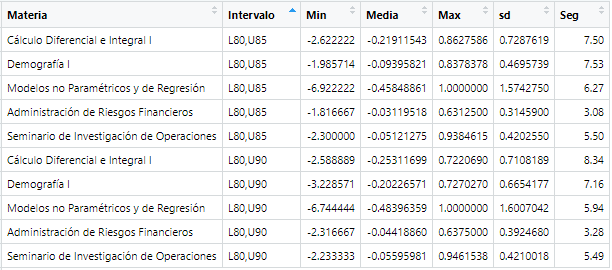
\includegraphics[scale = 0.9]{mat_med_dispersion} %width=\textwidth
\caption{\textit{Matriz con medidas de dispersión}}\label{matMedDispersion}
\end{figure}


Decidimos elegir $q_{1}$ y $q_{2}$ en base a la desviación estándar. Con la tabla \ref{matMedDispersion} obtuvimos una matriz de dos columnas que contine en su primer columna el intervalo y en la segunda el promedio de la desviación estándar para cada intervalo de las 5 materias. Los datos de dicha tabla los podemos ver en la figura \ref{promSD_5m_12p}.

%\begin{table}[H]
%\centering
% \begin{tabular}{|c|c|}
% \hline 
% Intervalo & Promedio\_sd \\ 
% \hline 
% L85,U80 & 0.6877112 \\ 
% \hline 
% L90,U80 & 0.6893502 \\ 
% \hline 
% L80,U85 & 0.7014912 \\ 
% \hline 
% L90,U85 & 0.7218125 \\ 
% \hline 
% L80,U90 & 0.7580821 \\ 
% \hline 
% L85,U90 & 0.7705116 \\ 
% \hline 
% L99,U90 & 0.8014339 \\ 
% \hline 
% L90,U99 & 0.9032661 \\ 
% \hline 
% L99,U80 & 0.9045421 \\ 
% \hline 
% L99,U85 & 0.9422762 \\ 
% \hline 
% L85,U99 & 0.9579213 \\ 
% \hline 
% L80,U99 & 0.9615854 \\ 
% \hline 
% \end{tabular} 
%\caption{\textit{Promedio de la desviación estándar}}\label{promSD_5m_12p_tabla}
%\end{table}


\begin{figure}[H]
\centering
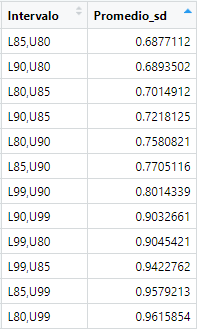
\includegraphics[scale = 1]{prom_SD_5m_12p} %width=\textwidth
\caption{\textit{Promedio de la desviación estándar: 5 materias, 12 pruebas}}\label{promSD_5m_12p}
\end{figure}


Los datos en la tabla \ref{promSD_5m_12p} están ordenados de menor a mayor con respecto al promedio de la desviación estándar. Para la segunda prueba se eligieron los primeros 6 intervalos de dicha tabla. Se eligieron 10 materias: \textit{Álgebra Lineal I}, \textit{Álgebra Superior II}, \textit{Algoritmos Genéticos}, \textit{Análisis Matemático IV}, \textit{Análisis Numérico}, \textit{Teoría de la Medida I}, \textit{Cálculo Diferencial e Integral IV}, \textit{Graficas y Juegos}, \textit{Inglés I} y \textit{Matemáticas Actuariales para Seguro de Daños}. La tabla con el promedio de la desviación estandar de sus datos se puede ver en la figura \ref{promSD_10m_6p}


\begin{figure}[H]
\centering
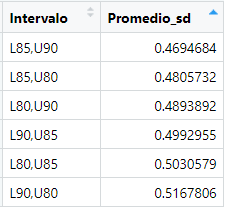
\includegraphics[scale = 1]{prom_SD_10m_6p} %width=\textwidth
\caption{\textit{Promedio de la desviación estándar: 10 materias, 6 pruebas}}\label{promSD_10m_6p}
\end{figure}


Para la tercera prueba elegimos, de la tabla \ref{promSD_10m_6p} los intervalos que tuvieran un promedio en la desviación estándar menor a $0.5$. Se eligieron otras 10 materias: \textit{Estadística III}, \textit{Teoría del Seguro}, \textit{Programación Entera}, \textit{Investigación de Operaciones}, \textit{Geometría Moderna I}, \textit{Geometría Analítica II}, \textit{Lógica Matemática I}, \textit{Cálculo Diferencial e Integral III}, \textit{Estadística I} y \textit{Bases de Datos}. La tabla con el promedio de la desviación estandar de sus datos se puede ver en la figura \ref{promSD_10m_4p}.


\begin{figure}[H]
\centering
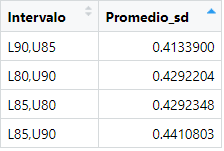
\includegraphics[scale = 1]{prom_SD_10m_4p} %width=\textwidth
\caption{\textit{Promedio de la desviación estándar: 10 materias, 4 pruebas}}\label{promSD_10m_4p}
\end{figure}

Podemos ver que los valores de la tabla \ref{promSD_10m_4p} son muy parecidos. Se hizo una prueba con los mismos intervalos pero con 5 materias que se dan en todos los semestres y además tienen muchos alumnos. La prueba se hizo para ver si habpía alguna diferencia en los datos y se pudiera elegir un sólo intervalo. Las materias que se eligieron para esta prueba fueron: \textit{Geometría Analítica I}, \textit{Cálculo Diferencial e Integral II}, \textit{Finanzas I}, \textit{Probabilidad II} y \textit{Procesos Estocásticos I}. La tabla con el promedio de la desviación estandar de sus datos se puede ver en la figura \ref{promSD_5m_4p}.


\begin{figure}[H]
\centering
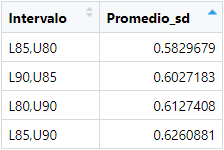
\includegraphics[scale = 1]{prom_SD_5m_4p} %width=\textwidth
\caption{\textit{Promedio de la desviación estándar: 5 materias, 4 pruebas}}\label{promSD_5m_4p}
\end{figure}

Analizando la información de las matrices de las figuras \ref{promSD_10m_4p} y \ref{promSD_5m_4p}, decidimos elegir los valores de $q_{1} = 85$ y $q_{2} = 80$. Por lo que el intervalo que buscamos estará formado por la cota inferior del intervalo de confianza al $85\%$ y por la cota superior del intervalo de confianza al $80\%$. Para visualizar de una mejor manera cómo se encuentra el intervalo formado, podemos ver la figura \ref{interConf}. De dicho intervalo vamos a obtener los valores para simular la demanda de alumnos.

\begin{figure}[H]
\centering
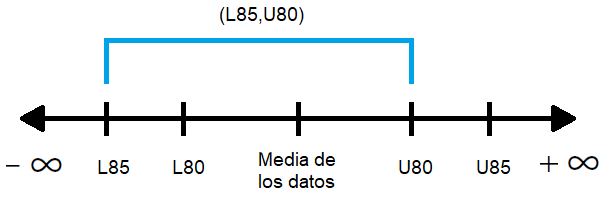
\includegraphics[scale = 0.7]{intervalos_confianza} %width=\textwidth
\caption{\textit{Diagrama de los intervalos de confianza}}\label{interConf}
\end{figure}

Finalmente con los valores de $q_{1} = 85$ y $q_{2} = 80$ se hizo una prueba aleatoria (eliminando la semilla). Las materias que elegimos para dicha prueba son: \textit{Estadística III}, \textit{Teoría del Seguro}, \textit{Cálculo Diferencial e Integral I}, \textit{Investigación de Operaciones}, \textit{Geometría Moderna I}, \textit{Geometría Analítica II}, \textit{Lógica Matemática I}, \textit{Cálculo Diferencial e Integral III}, \textit{Estadística I}, \textit{Bases de Datos}, \textit{Matemáticas Financieras}, \textit{Cálculo Diferencial e Integral II}, \textit{Probabilidad I}, \textit{Probabilidad II} y \textit{Procesos Estocásticos I}. Los resultados de la prueba aleatoria los podemos ver en la figura \ref{mat_med_dispersion_pruebaAl}. El promedio de la desviación estándar de todas las materias es $0.48$.%$0.4814898$.

\begin{figure}[H]
\centering
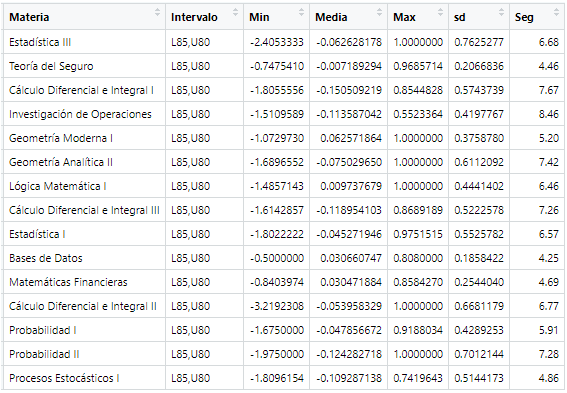
\includegraphics[scale = 0.9]{mat_med_dispersion_pruebaAleatoria} %width=\textwidth
\caption{\textit{Matriz con medidas de dispersión de prueba aleatoria}}\label{mat_med_dispersion_pruebaAl}
\end{figure}